\subsection{Empacotamento de \textit{plaintext} e \textit{ciphertext}}

Neste momento a seção 4 de \cite{lw23I} é tomada como base, cujo as 
operações foram implementadas em SageMath e C++. A única operação não implementeada foi a multiplicação entre criptogramas RGSW, afinal foge do escopo deste trabalho. A seguir, tome convenções necessárias para o resto do trabalho, tome $\rho = \varphi(p_2^{n_2})$, $\rho' = p_2^{n_2}$ com base $v_i$ e dual $v_i^{v}$; $\tau = \varphi(p_3^{n_3})$, $\tau' = p_3^{n_3}$ com base $w_i$ e dual $w_i^{v}$; $\delta_i^{(j)}$ representa a $i$-ésima componente do ruído da mensagem $\mu_i^{(j)}$ empacotada e cifrada em RGSW; $e_i^{(j)}$ é a $i$-ésima componente do ruído da mensagem $d_j$ resultante empacotada em RLWE.

\paragraph{Nota:} A única diferença da implementação para o proposto teoricamente é que para os plaintexts e ciphertexts, seus elementos vão ser armazenados sempre em $\mcR$ ao invés de ocasionalmente em $\mcR_1 \otimes \mcR_2^\vee \otimes \mcR_3$ ou $\mcR_1 \otimes \mcR_2 \otimes \mcR_3^\vee$. Por exemplo, para o criptograma  $a \in \mathcal{R}_1 \otimes \mathcal{R}_2^\vee \otimes \mathcal{R}_3$, vamos armazenar o criptograma $aP \in \mcR$ onde $P = \rho$. Esta multiplicação garante que o elemento tem representação única em $\mcR$ e facilita a implementação.

Surge uma dúvida natural, \textbf{Por que não empacotar as mensagens em um criptograma?}
O ruído acaba crescendo exponencialmente ao realizar múltiplos produtos externos consecutivamente. Emprestando um resultado da sessãoi seguinte, se decidirmos empacotar mensagens a expressão de um produto externo será: $Tr_{K/K_{13}} (e_1g^{-1}(c_2) + \mu_1 e_2) + e'$

Onde $e_1, e_2$ são os ruídos do criptograma RGSW e RLWE respectivamente. Como o ruído não possui nenhuma propriedade especial em relação as bases $v_i, w_i$ é válido afirmar que a sua norma vai crescer proporcional a um fator $\phi(p_2^{n_2})$. Portanto, após $k$ aplicações de produto externo, a norma final será limitada com um fator de $\approx \phi(p_2^{n_2})^{k/2} \phi(p_3^{n_3})^{k/2}$
que é exponencial. Tal crescimento pode ser verificado via o gráfico a seguir:

\begin{figure}[H]
    \centering
    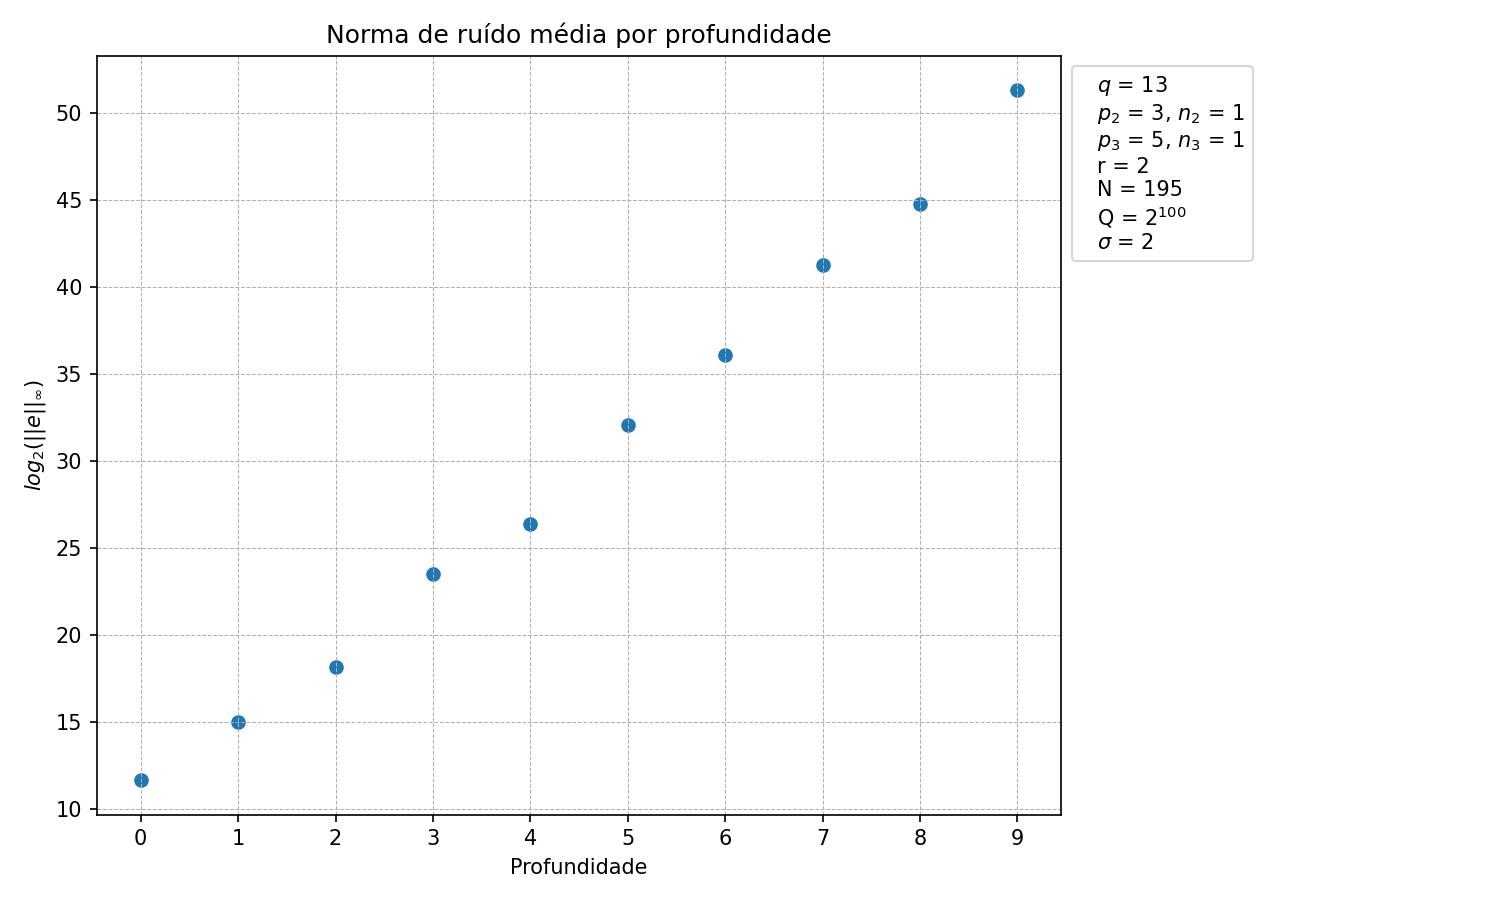
\includegraphics[width=0.7\textwidth]{sections/images/wrong_packing.jpg}
    \caption{Crescimento do ruído pela quantidade de produtos externos com empacotamento ingênuo.}
    \label{fig:wrong_packing}
\end{figure}
